\documentclass[10pt,twocolumn,letterpaper]{article}

\usepackage{cvpr}
\usepackage{times}
\usepackage{epsfig}
\usepackage{graphicx}
\usepackage{amsmath}
\usepackage{amssymb}
\usepackage{epstopdf}
\usepackage{multirow}
\usepackage{bbding}
\usepackage{colortbl}
\usepackage{subfigure}
\usepackage{float}


% Include other packages here, before hyperref.
\graphicspath{{figures}}
\newcommand{\argmax}{\operatornamewithlimits{argmax}}
\newcommand{\mtodo}[1]{{\bf \textcolor{blue}{[TODO: #1]}}}
\newcommand{\rev}[1]{{\textcolor{blue}{#1}}}
\newcommand{\dfun}[1]{{\llbracket #1 \rrbracket}}

% -------- Measure names --------
\newcommand{\J}{\mathcal{J}}
\newcommand{\F}{\mathcal{F}}
\newcommand{\T}{\mathcal{T}}

% If you comment hyperref and then uncomment it, you should delete
% egpaper.aux before re-running latex.  (Or just hit 'q' on the first latex
% run, let it finish, and you should be clear).
\usepackage[breaklinks=true,bookmarks=false]{hyperref}

\cvprfinalcopy % *** Uncomment this line for the final submission


%\def\cvprPaperID{****} % *** Enter the CVPR Paper ID here
\def\httilde{\mbox{\tt\raisebox{-.5ex}{\symbol{126}}}}

% Pages are numbered in submission mode, and unnumbered in camera-ready
%\ifcvprfinal\pagestyle{empty}\fi
\setcounter{page}{1}
\begin{document}

\title{Video Object Segmentation: A Survey}

\author{Zhixin Piao \quad Yongfei Liu \quad Qiong Huang \\
\small{School of Information Science and Technology, ShanghaiTech University}\\
{\tt\small \{piaozhx,liuyf,huangqiong\}@shanghaitech.edu.cn}
}

\maketitle

\begin{abstract}
Video object segmentation is more and more being of interest for computer vision and machine learning researchers.
Many applications on the rise need accurate and efficient segmentation mechanisms: autonomous driving, indoor navigation, 
and even virtual or augmented reality systems to name a few.
This demand coincides with the rise of deep learning approaches in almost every field or application target related to computer vision,
including video objects segmentation or scene understanding.


This paper provides a review on deep learning method for video objects segmentation in various setting, which can mainly be divided in semi-supervised and unsepervised manner. The huge difference between 
two setting is whether the first frame groundtruth is given in test phase.
Firstly, we address the important of video objects for many practical applications. Then, the popular deep learning archtectures and datasets are exposed  to help researchers have a big picture of 
video objects segmentation and an understanding of the efforts worked by former researchers.
Then we revise some existing methods which can tackle video objects segmenation successfully, and highlight their contributions and significance.
Finally, quantitative results are given for the described methods and the datasets in which they were evaluate, 
following up with a discussion of the results. 
At last, we point out a set of promising future works and draw our own conclusions about state-of-art video objects segmenation algorithms.




\end{abstract}

\section{Introduction}
Nowadays, semantic segmentation – applied to still 2D images, video, and even 3D or volumetric data

– is one of the key problems in the field of computer vision. Looking at the big picture, semantic segmentation is one of the high-level task that paves the way towards complete scene understanding. The importance of scene understanding as a core computer vision problem is highlighted by the fact that an increasing number of applications nourish from inferring knowledge from imagery. Some of those applications include autonomous driving [1] [2] [3], human-machine interaction [4], computational photography

[5], image search engines [6], and augmented reality to name a few. Such problem has been addressed in the past using various traditional computer vision and machine learning techniques. Despite the popularity of those kind of methods, the deep learning revolution has turned the tables so that many computer vision problems – semantic segmentation among them – are being tackled using deep architectures, usually Convolutional Neural Networks (CNNs) [7] [8] [9]

[10] [11], which are surpassing other approaches by a large margin in terms of accuracy and sometimes even efficiency. However, deep learning is far from the maturity achieved by other old-established branches of computer vision and machine learning. Because of that, there is a lack of unifying works and state of the art reviews. The ever-changing state of the field makes initiation difficult and keeping up with its evolution pace is an incredibly time-consuming task due to the sheer amount of new literature being produced. This makes it hard to keep track of the works dealing with semantic segmentation and properly interpret their proposals, prune subpar approaches, and validate results.

To the best of our knowledge, this is the first review to focus explicitly on deep learning for semantic segmentation. Various semantic segmentation surveys already exist such as the works by Zhu et al. [12] and Thoma [13], which do a great work summarizing and classifying existing methods, discussing datasets and metrics, and providing design choices for future research directions. However, they lack some of the most recent datasets, they do not analyze frameworks, and none of them provide details about deep learning techniques. Because of that, we consider our work to be novel and helpful thus making it a significant contribution for the research community.

The key contributions of our work are as follows:

(1) We provide a broad survey of existing datasets that might be useful for segmentation projects with deep learning techniques.

(2) An in-depth and organized review of the most significant methods that use deep learning for semantic segmentation, their origins, and their contributions.

(3) A thorough performance evaluation which gathers quantitative metrics such as accuracy, execution time, and memory footprint.

(4) A discussion about the aforementioned results, as well as a list of possible future works that might set the course of upcoming advances, and a conclusion summarizing the state of the art of the field.

The remainder of this paper is organized as follows. Firstly, Section 2 introduces the semantic segmentation problem as well as notation and conventions commonly used in the literature. Other background concepts such as common deep neural networks are also reviewed. Next, Section 3 describes existing datasets, challenges, and benchmarks. Section 4 reviews existing methods following a bottom-up complexity order based on their contributions. This section focuses on describing the theory and highlights of those methods rather than performing a quantitative evaluation. Finally, Section 5 presents a brief discussion on the presented methods based on their quantitative results on the aforementioned datasets. In addition, future research directions are also laid out. At last, Section 6 summarizes the paper and draws conclusions about this work and the state of the art of the field.
\section{Backgrounding}


\subsection{Common Deep Network BackBone}
\subsubsection{VGG}
VGG
\subsubsection{ResNet}
ResNet


\subsection{Common Deep Network Architecture}

\subsubsection{FCN}
FCN


\subsubsection{SegNet}
SegNet

\subsubsection{U-Net}
U-Net


\subsubsection{DeepLab}
DeepLab

\subsection{Common Method for Video}

\subsubsection{Optical Flow}
Optical Flow

\subsection{Common Method for One-Shot}

\subsubsection{Fine-Tune}
Fine-Tune

\subsubsection{Mask Warp}
Fine-Tune
\section{Datasets}
Throught the years,  there are so many excellent video segmentation datasets
\subsection{Datasets}

\paragraph{DAVIS}

Densely-Annotated VIdeo Segmentation is a  difficult challenge, which is mainly purposed for video object segmentation.
Frame resolution varies across sequences but all of them were downsampled to 480 p for the challenge. 
Pixel-wise annotations are provided for each frame for four different categories: human, animal, vehicle, and object.
DAVIS-2016 \cite{DAVIS2016}is composed by 50 high-definition sequences which add up to 2079 and 1376 frames for training and validation respectively.
This dataset mainly addresses problem on primary objects segmentaion, which means that there are at least one target foreground object in videos.
DAVIS-2017 \cite{DAVIS2017} have extended the number of sequences to 90, which is 60 sequences for training and 30 for validation, which contains 4209 and 1999 frames respectively.
They segment the main moving objects in the scene and divide them by their semantic, even though they might have the same motion. So we can refer DAVIS-2017 as the video instance segmentations.

\begin{figure}[ht]
    \centering
    \begin{subfigure}{}
        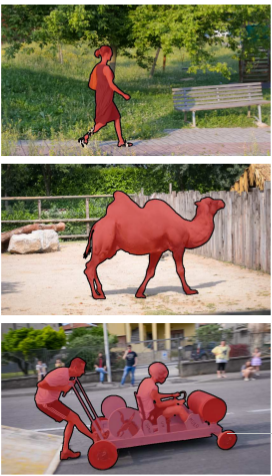
\includegraphics[width=0.2\textwidth]{figure/Davis_primary1.png}  
    \end{subfigure}
    \begin{subfigure}{}
        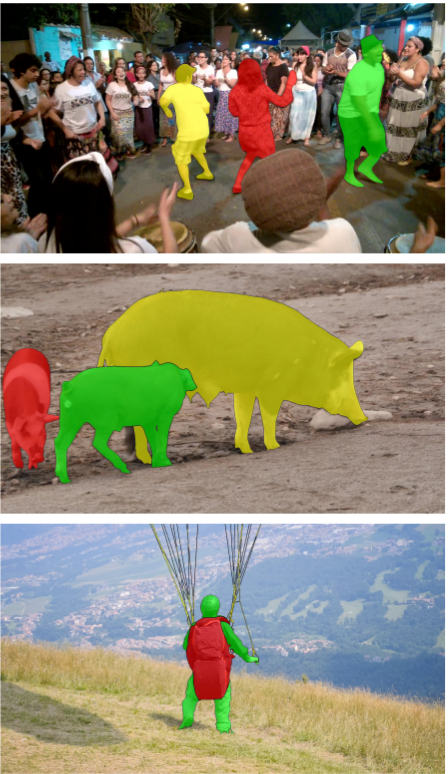
\includegraphics[width=0.2\textwidth]{figure/Davis_instance2.png}
    \end{subfigure}
    \caption{DAVIS dataset. The left is foreground segmentaion setting. The right is instance segmentation setting}
% 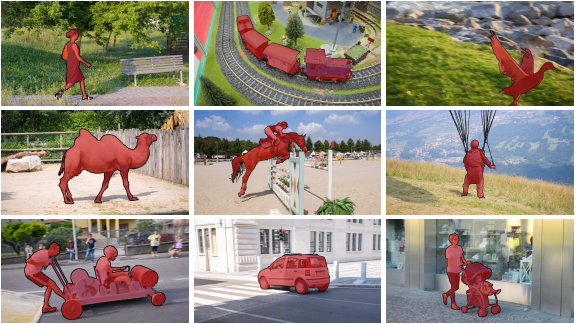
\includegraphics[width=0.45\textwidth]{figure/Davis_primary.png}    
\end{figure}




\paragraph{Youtube-Objects~\cite{Youtube}} 
The Youtube-Objects is a database of videos collected from YouTube which contain objects from ten PASCAL VOC classes: 
aeroplane, bird, boat, car,cat, cow, dog, horse, motorbike, and train.
That database does not contain pixel-wise annotations but Jain et al 
manually annotated a subset of 126 video sequences.
They took every 10th frame from those sequences and generated semantic labesl. 
That totals 10167 annotated frames at $480\times 360$ pixels resolution.

\paragraph{SegTrack-v2~\cite{SegTrack}}
The dataset is an updated version of the SegTrack dataset, which provide more additional
annotations of objects for other individual objects. The total 14 videos contain 1066 frames with pixel-
level annotations. 






\section{Methods}

\subsection{Semi-supervised VOS}
test
% Single Object

% \mtodo{Sort by IoU: 
% 	LucidTracker~\cite{LucidTracker}, 
% 	OnAVOS~\cite{OnAVOS},
% 	OSVOS$^\text{S}$~\cite{OSVOS-S}, 
% 	SGV~\cite{SGV},
% 	MaskRNN~\cite{MaskRNN},
% 	OSVOS~\cite{OSVOS}, 
% 	MSK~\cite{MSK},
% 	OSMN~\cite{OSMN}, 
% 	SFL~\cite{SFL}, 
% 	CTN~\cite{CTN}, 
% 	VPN~\cite{VPN}, 
% 	PLM~\cite{PLM}, 
% 	OFL~\cite{OFL}, 
% 	BVS~\cite{BVS}, 
% 	FCP~\cite{FCP}, 
% 	JMP~\cite{JMP}, 
% 	HVS~\cite{HVS}, 
% 	SEA~\cite{SEA} 
% }


% Mutliple Objects


% \mtodo{Sort by IoU: 
% 	DyeNet~\cite{DyeNet}, 
% 	MaskRNN~\cite{MaskRNN}, 
% 	OSVOS~\cite{OSVOS}, 
% 	OSMN~\cite{OSMN}, 
% 	LucidTracker~\cite{LucidTracker},
% 	OSVOS$^\text{S}$~\cite{OSVOS-S},
% 	MSK~\cite{MSK},
% }

\subsection{Unsupervised VOS}
Video object segmentation is the task of extracting spatio-temporal regions that correspond to object moving in at
least one frame in the video sequence. In contrast to semi-supervised VOS, unsupervised video object segmentation have 
more challages and is more practical in real world. In real world case, with the limitation of resources and the diversity of scenario,
it is difficult to simulate various outdoor scenario and collect dataset from it in laboratory. So unsupervised video object 
segmentation have more important impact on our real daily life. To better understand to unsupervised setting, here we list some
obvious difference between semi-supervised video segmentation.
\begin{enumerate}
    \item no first frame groundtruth is provided in test phase.
    \item no finetune process in test phase is needed.
\end{enumerate}

In unsupervised VOS tasks, we can regard them as zero-shot video objects segmentation. Because we cannot have any objects priors
in test phase, namely that the objects in testset does not exit in training phase. The task's main challages is that we need to infer
the primary objects which are moving in video frames automatically. The algorithm can discovers the most salient, or primary, objects,
that move against a video's background or display different color statistics. To better capture the moving objects against the background,
the object motion is the critical cue for identify salients objects throught entire video sequences. Next, we will introduce some important
methods which is commonly used in unsupervised VOS.

\subsubsection{Motion in Video Sequences}
In traditional static image semantic segmentation, the apperance information play an import role, which means that 
the performance is enough good if we can extract more reliable apperance features. But in video setting, thera are various
difficult challlenges caused by object moving, which are motion blur and ambigious and occluated. We just rely on apperance information
, which can  fail in this specifical scenario. Motion information can greatly help reduce this ambigious. We can capture more temporal information
to help locate objects in videos frames.

Jain $et.al$ \cite{Jain2017FusionSeg} propose an end-to-end learning framework for segmenting generic objects in video,
which learns to combine appearance and motion information to produce pixel level segmentation masks for all prominent objects.
They design a two-stream fully convolutional neural network which fuses together motion and apperance in a unified framework.
\begin{figure}[ht]
    \centering
    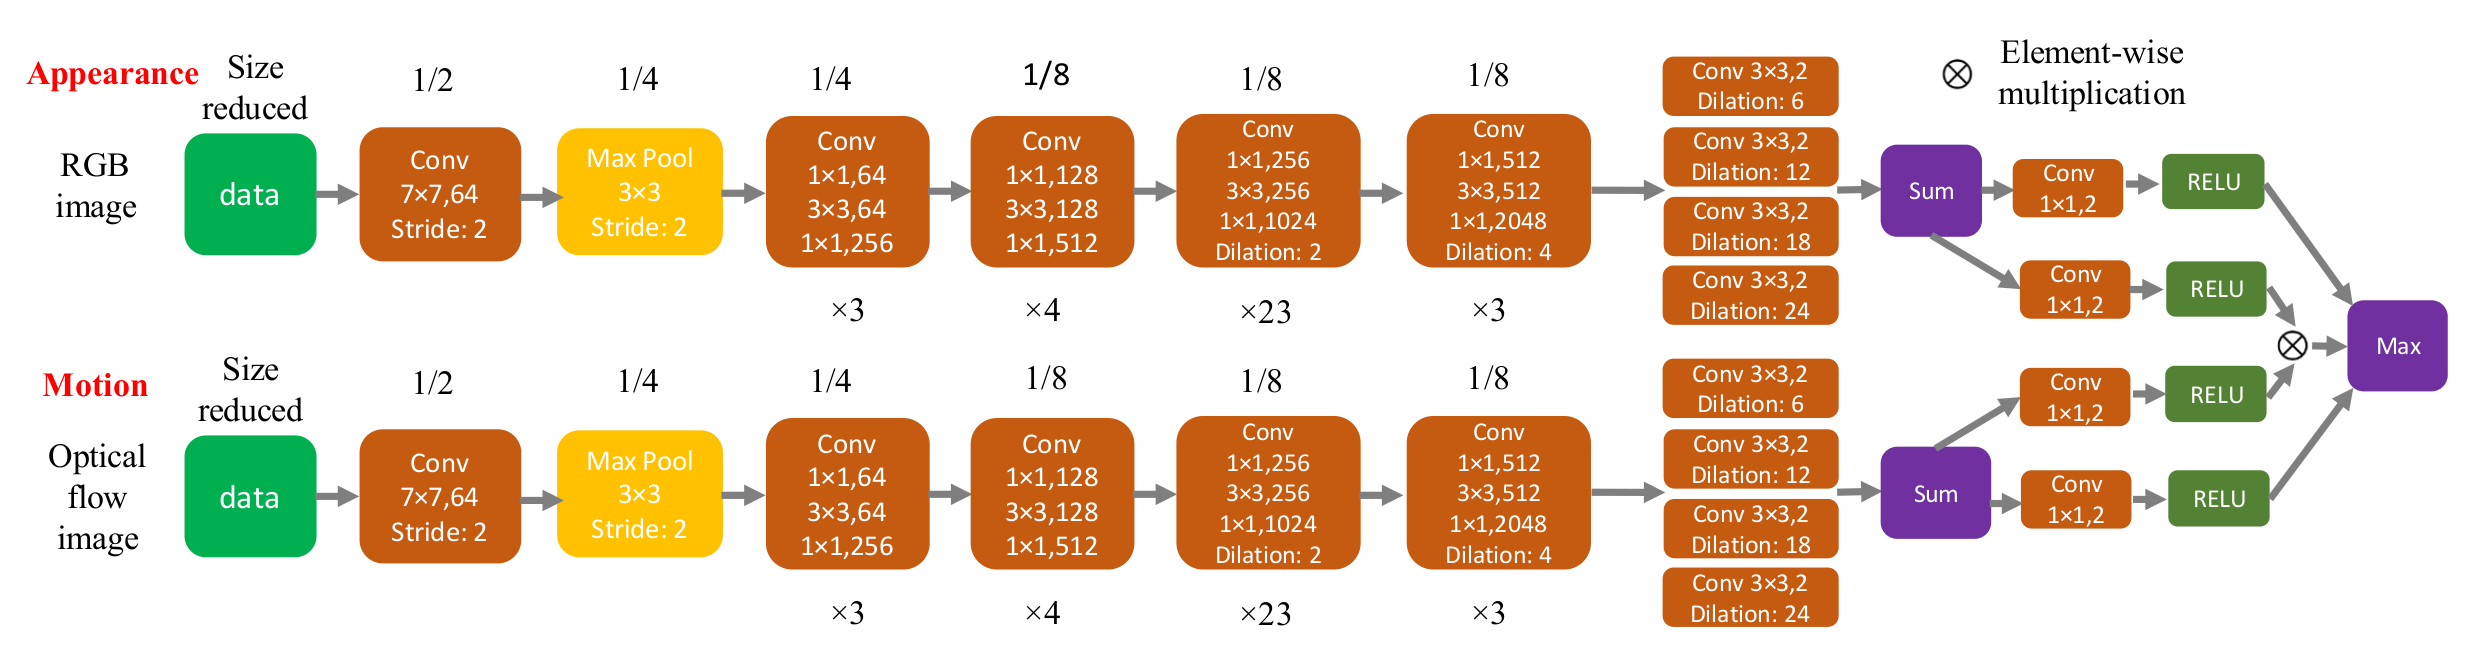
\includegraphics[width=0.5\textwidth]{./figure/FSEG_NET.png}
    \caption{FSEG Network}
    \label{FSEG}
\end{figure}

As shown in Fig \ref{FSEG}, the network can take two different inputs, which are raw images and optical flow images respectively.
The motion branch can map the motion into foreground objects, which can greatly capture temporal infomation.
In the last fusion stage, this method does not simply concat two stream feature to get the final prediction.
They design a new fusion strategy to create three independent parallel branches. They apply $1\times1$ convolution to apperance and
motion branch. Finally they apply a layer that thkes the elements-wise maximum to obtain the final prediction. The movivation is that 
an object segmentation prediction is reliable if 1) either apperance or motion model along predicts the object 
segmentation with very strong confidence or 2) their combination together predicts the segmentation with high confidence. 

Besides the two stream strategy, 




% \mtodo{Sort by IoU:
% 	% IET~\cite{li2018instance}, 
% 	ARP~\cite{koh2017}, 
% 	LVO~\cite{tokmakov17}, 
% 	FSEG~\cite{jain2017}, 
% 	LMP~\cite{tokmakov2017}, 
% 	SFL~\cite{cheng2017sfl}, 
% 	FST~\cite{papazoglou2013}, 
% 	CUT~\cite{keuper2015}, 
% 	NLC~\cite{faktor2014}, 
% 	MSG~\cite{ochs2011}, 
% 	KEY~\cite{lee2011}, 
% 	CVOS~\cite{taylor2015},
% 	TRC~\cite{fragkiadaki2012}
% }

\section{Discussion}

\subsection{Evaluation Metrics}
In a supervised evaluation framework, given a groundtruth mask $G$ on a particular frame and an output segmentation $M$,
any evaluation measure ultimately has to answerthe question how well $M$ fits $G$. As justified in \cite{pont2016supervised}, 
for images one can use two complementary points of view, regionbased and contour-based measures. As videos extends the
dimensionality of still images to time, the temporal stability of the results must also be considered.


\begin{table*}[ht]
	\begin{center}
		\setlength\tabcolsep{1pt}
		\begin{tabular}{|c|c|c|c|c|c|c|c|c|c|c|}
		\hline
Dataset& Metrics &OSVOS~\cite{OSVOS} &$\text{OSVOS}^\text{S}$\cite{OSVOS-S} &BVS\cite{BVS} &PML~\cite{PML} &Lucid~\cite{LucidTracker} &CTN~\cite{CTN} &MaskRNN\cite{MaskRNN} &OSMN\cite{OSMN} &DyeNet~\cite{DyeNet} \\
\hline
\multirow{2}{*}{DAVIS2016} &$\J$ mean  &79.8 &85.6 & 60.0 &86.1 &\textbf{91.2} &73.5 &80.4 &74 &86.2 \\
\cline{2-11}
&$\F$ Mean  &80.6 &86.4 &58.8 &-- &\textbf{94.2} &69.3 &82.3 &-- &-- \\
\hline
\multirow{2}{*}{DAVIS2017} &$\J$ mean  &55.1 &-- &-- &-- &65.1 &-- &60.5 &52.5 &\textbf{67.3} \\
\cline{2-11}
&$\F$ Mean &62.1 &-- &-- &-- &70.6 &-- &-- &57.1 &\textbf{71}\\
\hline
\end{tabular}
\end{center}
\caption{The result of semi-supervised methods on DAVIS datasets.}
\label{table:semisuperivsed_all_dataset}
\end{table*}


\begin{table*}[ht]
	\begin{center}
		\setlength\tabcolsep{3pt}
		\begin{tabular}{|c|c|c|c|c|c|c|}
		\hline
Dataset& Metrics &FSEG~\cite{Jain2017FusionSeg}  &LVO~\cite{Tokmakov2017Learning} &LMP~\cite{Tokmakov2017Learning} & POS~\cite{Koh2017Primary} &IET~\cite{li2018instance}\\
\hline
\multirow{2}{*}{DAVIS2016} &$\J$ mean  &71.51   &75.9     &69.7       &76.3    &78.5\\
\cline{2-7}
&$\F$ Mean      &   --    &72.1  &66.3        &71.1      &75.5\\
\hline
\end{tabular}
\end{center}
\caption{The result of unsupervised methods on DAVIS datasets.}
\label{table:unsuperivsed_all_dataset}
\end{table*}




\subsubsection{Accuracy}
\paragraph{Region Similarity $\J$}
To measure the region-based segmentation similarity, i.e. the number of mislabeled pixels,
one employ the Jaccard index $\J$ defined as the intersectionover-union of the estimated segmentation and the groundtruth mask.
The Jaccard index has been widely adopted since its first appearance in PASCAL VOC2008 \cite{martin2004learning}, 
as it provides intuitive, scale-invariant information on the number of mislabeled pixels. Given an output segmentation $M$ and 
the corresponding ground-truth mask $G$ it is defined as $\J = \frac{|M \cap G|}{|M\cup G|}$

\paragraph{Contour Accuracy $\F$}
From a contour-based perspective, one can interpret $M$ as a set of closed contours $c(M)$
delimiting the spatial extent of the mask. Therefore, one
can compute the contour-based precision and recall $Pc$ and
$Rc$ between the contour points of $c(M)$ and $c(G)$, via a bipartite graph matching in order to be robust to small inaccuracies,
as proposed in \cite{martin2004learning}.
So the F-measure $F$ is a good trade-off between two, which is  defined as $F = \frac{2Pc Rc}{Pc+Rc}$.

\paragraph{Temporal Stability $\T$}
Temporal stability $\T$. Intuitively, $\J$ measures how well the pixels of the two masks match, while $F$ measures the
accuracy of the contours. However, temporal stability of the results is a relevant aspect in video object segmentationsince the evolution of object shapes is an important cue for
recognition and jittery, unstable boundaries are unacceptable in video editing applications. 



\subsection{Results}
As shown in Table\ref{table:unsuperivsed_all_dataset},\ref{table:semisuperivsed_all_dataset} we can compare the performance of difference algorithm. In generally, the method based on deep learning would excel the the traditional 
methods.The method combined spatial-temporal information can greatly help improve performance in paper\cite{Tokmakov2017Learning}. And in normal case, optical flow method can help capture the 
temporal information, but it is still not powerful enough. The visual memory module applied in temporal can help improve $4.4\%$ in $\J$ evaluation metrics. Let us see some traditional methods,like
\cite{Koh2017Primary,li2018instance}, they can also gain impressive performance in DAVIS dataset because they can design some specifical feature to model sequences data. Li $et.al$ use instance embedding method
to force the algorithm to learn the instance concepts. So they can get excellent performance in instance segmentation setting.



\section{Conclusion}


{\small
\bibliographystyle{ieee}
\bibliography{reference}
}


\end{document}
